%\VignetteIndexEntry{An R Package for RTF output}
%\VignetteDepends{R.oo, gsubfn}
%\VignetteSuggests{ggplot2, lattice, grid}
%\VignetteImports{}
%\VignettePackage{rtf}
%\VignetteKeyword{RTF}
%\VignetteKeyword{Microsoft Word}

\documentclass[11pt,letterpaper]{article}
\usepackage{Sweave}
\usepackage[hidelinks]{hyperref}
\usepackage{geometry}
\geometry{hmargin = 1.5in, vmargin = 1.5in }
    % Keeps comments in the R code.
\pagestyle{plain}


\begin{document}
\Sconcordance{concordance:rtf.tex:rtf.Rnw:%
1 35 1 1 2 4 0 1 2 3 1 1 2 1 0 1 2 1 0 1 4 5 0 1 2 8 1 1 3 5 0 1 2 2 1 %
1 2 4 0 1 2 3 1 1 2 1 0 4 1 3 0 1 2 4 1 1 2 4 0 1 2 8 1 1 2 4 0 1 2 2 1 %
1 2 4 0 1 2 3 1 1 2 4 0 1 2 17 1 1 2 4 0 1 2 1 1 1 2 4 0 1 2 16 1 1 2 1 %
0 1 1 3 0 1 2 1 3 15 0 2 2 4 0 1 2 3 1 1 2 1 0 1 1 3 0 2 2 12 0 1 2 1 1 %
1 3 5 0 1 2 7 1 1 2 4 0 1 2 4 1 1 2 5 0 1 2 2 1 1 2 4 0 1 2 2 1 1 6 5 0 %
1 2 4 0 1 2 2 1 1 2 4 0 1 2 5 1 1 2 1 0 2 1 4 0 1 2 2 1 1 2 4 0 1 2 3 1 %
1 2 1 0 1 1 4 0 2 2 4 0 1 2 1 1 1 2 1 0 1 1 5 0 1 3 1 2 4 0 1 2 5 1 1 3 %
2 0 2 1 4 0 1 2 5 1 1 2 4 0 1 2 4 1 1 2 4 0 1 2 4 1 1 2 1 0 1 1 1 2 2 1 %
3 0 1 2 4 1 1 2 1 0 1 2 1 1 3 0 1 2 3 1}


\title{Vignette for the \texttt{rtf} Package}
\author{Michael E. Schaffer}
\date{June 2012}
\maketitle

\tableofcontents

\section{Introduction}

\texttt{rtf} is a package for outputting Rich Text Format (RTF) files with high resolution tables and graphics that may be edited with standard word processors.  This package is not meant as a substitute for \texttt{Sweave}, but as a simpler alternative that produces reports compatible with Microsoft Word and other popular word processors.  This vignette demonstrates some of the functions in a larger context than the help file examples.


\section{Usage}

First, load the package.

\begin{Schunk}
\begin{Sinput}
> library(rtf)
\end{Sinput}
\end{Schunk}


Now, we can use the \texttt{RTF} function to initialize an RTF object and return a reference for all subsequent methods.  You may notice that the parameters for this method are similar to those used in \texttt{base} plots.  We can define the RTF page width and height (in inches), the default font size (in points), and the outer page margins (in inches).

\begin{Schunk}
\begin{Sinput}
> output<-"rtf_vignette.doc"   # although this is RTF, we can use the
>                              # .doc extension so it opens in MS Word
> rtf<-RTF(output,width=8.5,height=11,font.size=10,omi=c(1,1,1,1))
> # Other rtf commands here...
> 
> done(rtf)                    # writes and closes the file
\end{Sinput}
\end{Schunk}



\section{Text}

\subsection{Basic Text}
There are three ways to output text to an RTF document: \texttt{addHeader}, \texttt{addParagraph}, \texttt{startParagraph}/\texttt{addText}/\texttt{endParagraph}.  These are very similar, but some differences are outlined below.

First, we can create a new section with a title in bold followed by either a subtitle or the section text in normal text.
\begin{Schunk}
\begin{Sinput}
> addHeader(rtf,title="Section Header",
+ 	      subtitle="This is the subheading or section text.")
\end{Sinput}
\end{Schunk}


If a header is not necessary, a self-contained paragraph can be created with the \texttt{addParagraph} method.
\begin{Schunk}
\begin{Sinput}
> addParagraph(rtf,"This is a new self-contained paragraph.\n")
\end{Sinput}
\end{Schunk}


Alternatively, we may define a paragraph start and end.  Text may be inserted between these methods using the \texttt{addText} function.

\begin{Schunk}
\begin{Sinput}
> startParagraph(rtf)
> addText(rtf,"This text was added with the addText command.  ")
> addText(rtf,"You can add styled text too.  ",bold=TRUE,italic=TRUE)
> addText(rtf,"You must end the paragraph manually.")
> endParagraph(rtf)
\end{Sinput}
\end{Schunk}


\subsection{New Lines}
There are a couple ways to insert new lines within the text.  First, you may use ``\texttt{\textbackslash n}'' within any string.  Alternatively, you may insert a new line using the \texttt{addNewLine} function.

\begin{Schunk}
\begin{Sinput}
> addNewLine(rtf)
\end{Sinput}
\end{Schunk}




\subsection{Unicode and Greek Characters}
Uppercase and lowercase Greek characters may be used in any string but must be encoded in a specific manner.  The implementation mimics syntax used for encoding Unicode characters in HTML 4.0.  

For example, to export uppercase Alpha through Epsilon, we can use the follow code.

\begin{Schunk}
\begin{Sinput}
> addParagraph(rtf,"&Alpha; &Beta; &Gamma; &Delta; &Epsilon;\n\n")
\end{Sinput}
\end{Schunk}

For lowercase, we use the following.

\begin{Schunk}
\begin{Sinput}
> addParagraph(rtf,"&alpha; &beta; &gamma; &delta; &epsilon;\n\n")
\end{Sinput}
\end{Schunk}


Other Unicode characters are supported through specific HTML equivalents.  These are defined at \url{http://www.w3.org/TR/html4/sgml/entities.html}.  Unicode characters may be encoded directly using the Unicode decimal value.  For example, to encode three heart shapes, we use the following combination of Unicode and RTF syntax. 

\begin{Schunk}
\begin{Sinput}
> addParagraph(rtf,"\\u9829\\3 \\u9829\\3 \\u9829\\3\n\n")
\end{Sinput}
\end{Schunk}


\subsection{URLs}
URLs are not currently supported, but will be in a future version.







\subsection{Mathematical Formulae}
Unfortunately, support for mathematical formulae is not part of the RTF specification.  This package is not recommended for heavy use of formulae and cannot produce output on par with \texttt{Sweave}.


\subsection{RTF Code}
Native RTF may be used directly within any text block buy simply adding a backslash to the RTF commands.  For example, the following demonstrates two ways to style bold text using native RTF commands, ``\texttt{\textbackslash b}'' and ``\texttt{\textbackslash b0}''.  The full RTF specificaiton of RTF syntax is available at \url{http://www.microsoft.com/en-us/download/details.aspx?id=10725}.

\begin{Schunk}
\begin{Sinput}
> addParagraph(rtf,"Normal, \\b this is bold\\b0, normal.\n")
\end{Sinput}
\end{Schunk}

or alternatively, with curly brackets to contain the code,
\begin{Schunk}
\begin{Sinput}
> addParagraph(rtf,"Normal, {\\b\\i bold-italic}, normal.\n")
\end{Sinput}
\end{Schunk}

When incorporating native RTF code, it is important to pay attention to spacing in the RTF syntax.  Improper spacing can cause MS Word parser errors that are difficult to debug.


\section{Formatting}
Currently, document formatting with the \texttt{rtf} package functions is limited.  There are, however, a few useful methods.  In addition, all of the native RTF syntax is available for more complex document formatting.

Three functions that allow changes in text placement include: \texttt{increaseIndent} to indent text or figures, \texttt{decreaseIndent} to move the indentation to the left, and \texttt{addPageBreak} that allows changes in page orientation and margins in the middle of a document.



\section{Tables}
The \texttt{addTable} function may be used to add tabular data to an RTF report from a \texttt{data.frame} or any data that can be coerced to a \texttt{data.frame}.  For tables with specific formatting requirements, it is recommended to format the table data before passing to the \texttt{addTable} function.  This function will guess the best column widths to use, but also allows the user to specify column widths.


For example we can insert a table based on the \texttt{iris} data below.

\begin{Schunk}
\begin{Sinput}
> tab<-as.data.frame(head(iris)) # create a data.frame
> colnames(tab)<-gsub("\\."," ",colnames(tab)) # format column names
\end{Sinput}
\end{Schunk}

% latex table generated in R 3.0.2 by xtable 1.7-1 package
% Mon Jan  6 09:19:22 2014
\begin{table}[!htbp]
\centering
\begin{tabular}{rrrrrl}
  \hline
 & Sepal Length & Sepal Width & Petal Length & Petal Width & Species \\ 
  \hline
1 & 5.10 & 3.50 & 1.40 & 0.20 & setosa \\ 
  2 & 4.90 & 3.00 & 1.40 & 0.20 & setosa \\ 
  3 & 4.70 & 3.20 & 1.30 & 0.20 & setosa \\ 
  4 & 4.60 & 3.10 & 1.50 & 0.20 & setosa \\ 
  5 & 5.00 & 3.60 & 1.40 & 0.20 & setosa \\ 
  6 & 5.40 & 3.90 & 1.70 & 0.40 & setosa \\ 
   \hline
\end{tabular}
\end{table}
\begin{Schunk}
\begin{Sinput}
> addTable(rtf,tab,font.size=9,row.names=FALSE,NA.string="-")
\end{Sinput}
\end{Schunk}



We may also want to output a table from the \texttt{table} command, such as the following.
\begin{Schunk}
\begin{Sinput}
> tab<-table(iris$Species,floor(iris$Sepal.Length))
> names(dimnames(tab))<-c("Species","Sepal Length")
\end{Sinput}
\end{Schunk}

% latex table generated in R 3.0.2 by xtable 1.7-1 package
% Mon Jan  6 09:19:22 2014
\begin{table}[!htbp]
\centering
\begin{tabular}{rrrrr}
  \hline
 & 4 & 5 & 6 & 7 \\ 
  \hline
setosa &  20 &  30 &   0 &   0 \\ 
  versicolor &   1 &  25 &  23 &   1 \\ 
  virginica &   1 &   6 &  31 &  12 \\ 
   \hline
\end{tabular}
\end{table}
Here we can specify the columns widths and a string to substitute for \texttt{NA} values.
\begin{Schunk}
\begin{Sinput}
> addTable(rtf,tab,font.size=10,row.names=TRUE,NA.string="-",
+              col.widths=c(1,0.5,0.5,0.5,0.5) )
\end{Sinput}
\end{Schunk}


\section{Figures}
Figures and graphics may be inserted into the RTF document as easily as text.  One limitation of the RTF specification is that vector-based image formats (e.g. EPS or PDF) are undefined except for Microsoft's proprietary WMF and EMF formats.  For this reason the \texttt{rtf} package uses raster-based PNG files for inserting figures into RTF documents.  The resolution for these images may be set to any value; however, for publication, it is recommended that users independently export figures as PDF.


The basic approach for adding plots is the \texttt{addPlot} function.  This command takes a plot function as a paramater, along with specific RTF parameters, and then any other parameters to be sent to the plot function.  The syntax is as follows, where ``\texttt{...}'' represents all parameters to be passed to the \texttt{plot.fun} function.  Notice how we define the plot width and height (in inches), along with the desired resolution (in dots per inch).

\begin{Schunk}
\begin{Sinput}
> addPlot(RTF.object, plot.fun=plot.fun, width=4, height=5, res=300, ...)
\end{Sinput}
\end{Schunk}


\subsection{\texttt{base} Plots}
For \texttt{base} graphics plots, we can use the \texttt{addPlot} in two ways.  First we can directly use the plot function in the \texttt{addPlot} function.  Below, we simply use \texttt{R}'s \texttt{plot} function.

\begin{Schunk}
\begin{Sinput}
> plot(iris[,1],iris[,2])
\end{Sinput}
\end{Schunk}
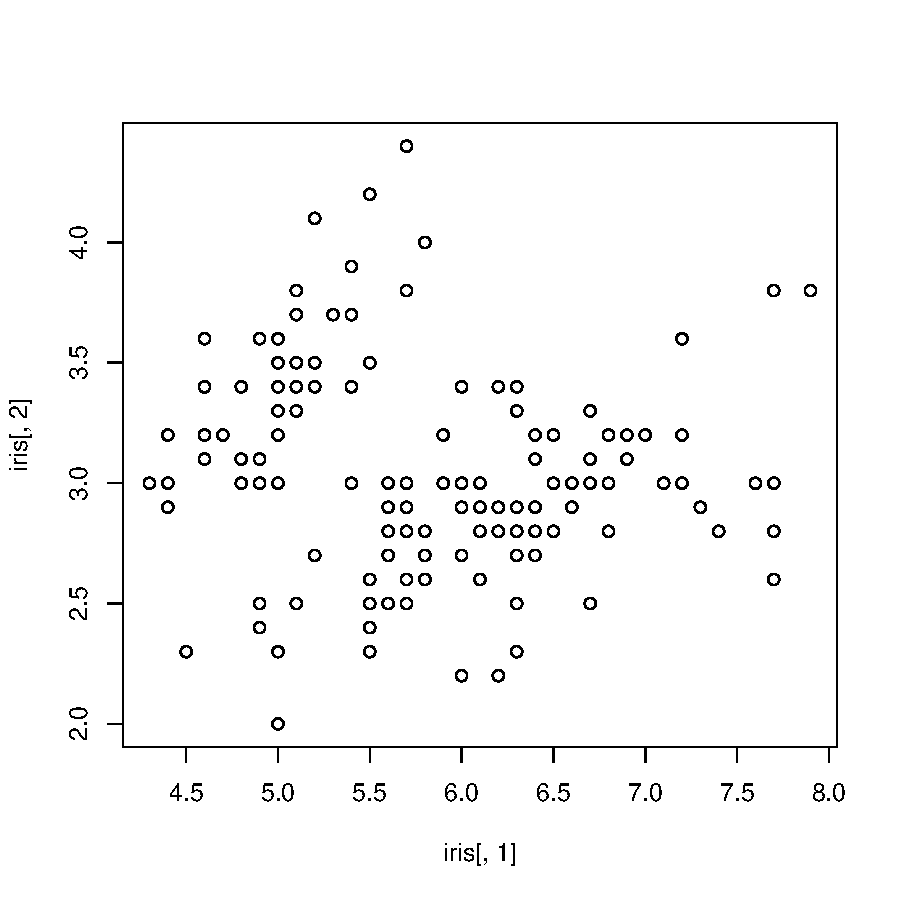
\includegraphics{rtf-019}

To add this plot to the document, we use the following.

\begin{Schunk}
\begin{Sinput}
> addPlot(rtf,plot.fun=plot,width=6,height=6,res=300, iris[,1],iris[,2])
\end{Sinput}
\end{Schunk}

Alternatively, we can wrap a more complex plot that has several steps into a function that takes any number of parameters.

\begin{Schunk}
\begin{Sinput}
> newPlot<-function() {
+ 	par(pty="s",cex=0.7)      # adjust plot style
+ 	plot(iris[,1],iris[,2])
+ 	abline(h=2.5,v=6.0,lty=2) # add some lines
+ }
> newPlot()
\end{Sinput}
\end{Schunk}
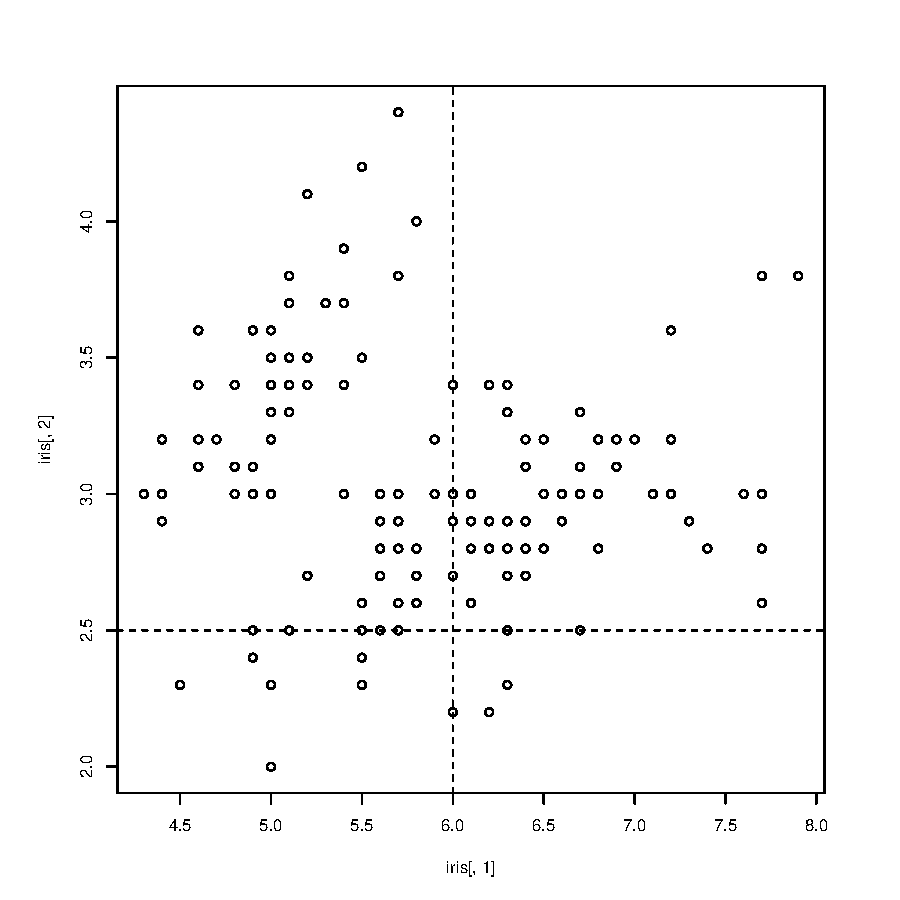
\includegraphics{rtf-021}

Then we add this plot to the document with the following.  Note in this case there are no extra \texttt{plot.fun} parameters to pass along, but the function may be rewritten to accept any parameters to promote reuse of plotting code.

\begin{Schunk}
\begin{Sinput}
> addPlot(rtf,plot.fun=newPlot,width=6,height=6,res=300)
\end{Sinput}
\end{Schunk}


\subsection{\texttt{lattice} Plots}
The \texttt{lattice} package enables trellis plots for visualizing relationships between variables of complex data sets.  To create the output for RTF, we just assign the \texttt{lattice} plot to a variable.  The \texttt{print} function may then be used to visualize the plot.


\begin{Schunk}
\begin{Sinput}
> library(lattice)
> p <- histogram( ~ height | voice.part, data = singer, xlab="Height")
> print(p)
\end{Sinput}
\end{Schunk}
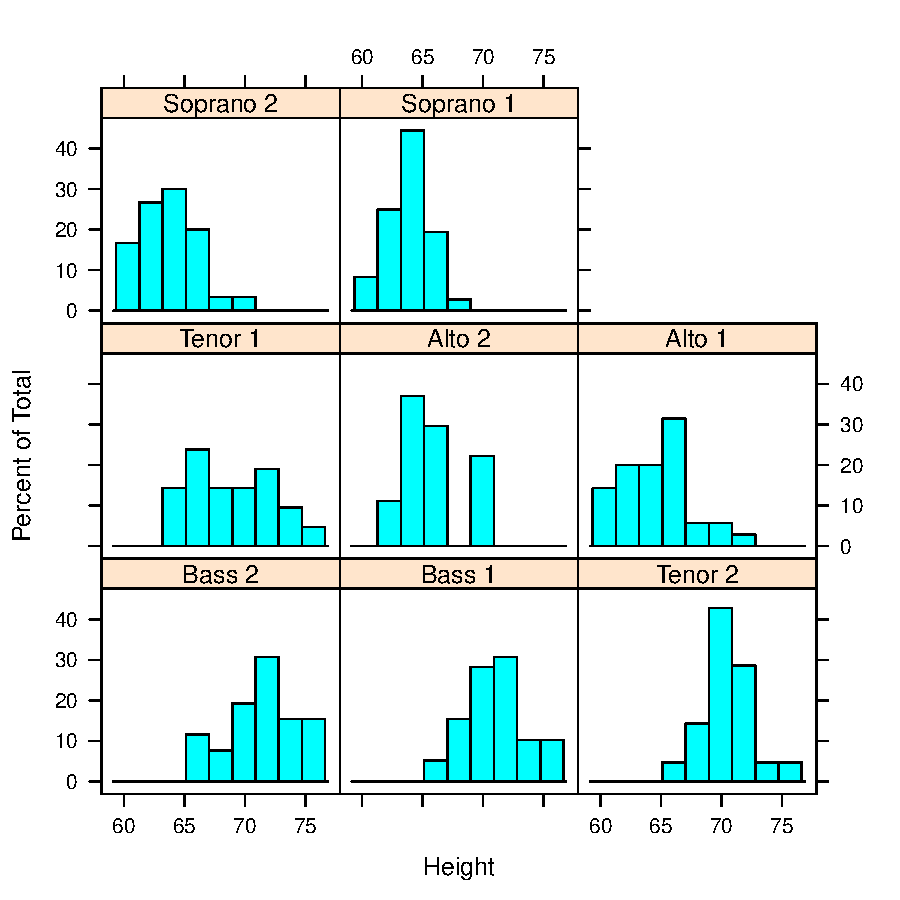
\includegraphics{rtf-023}

To include this plot in the RTF document we again call the \texttt{addPlot} method.  However, for \texttt{lattice} plots, we pass \texttt{print} as the \texttt{plot.fun} function and use the \texttt{p} variable as a parameter for this function.  Below is an example that specifies the plot width and height (in inches), along with the desired resolution (in dots per inch).

\begin{Schunk}
\begin{Sinput}
> addPlot(rtf,plot.fun=print,width=5,height=5,res=300,p)
\end{Sinput}
\end{Schunk}


Alternatively, we can use the \texttt{addTrellisObject} method with \texttt{lattice} plots.  The \texttt{addTrellisObject} method is suited for multi-page trellis objects and will create an image for each page in the RTF document.  It also works for single page images as well.

\begin{Schunk}
\begin{Sinput}
> p2 <- densityplot( ~ height | voice.part, data = singer, xlab = "Height")
> print(p2)
\end{Sinput}
\end{Schunk}
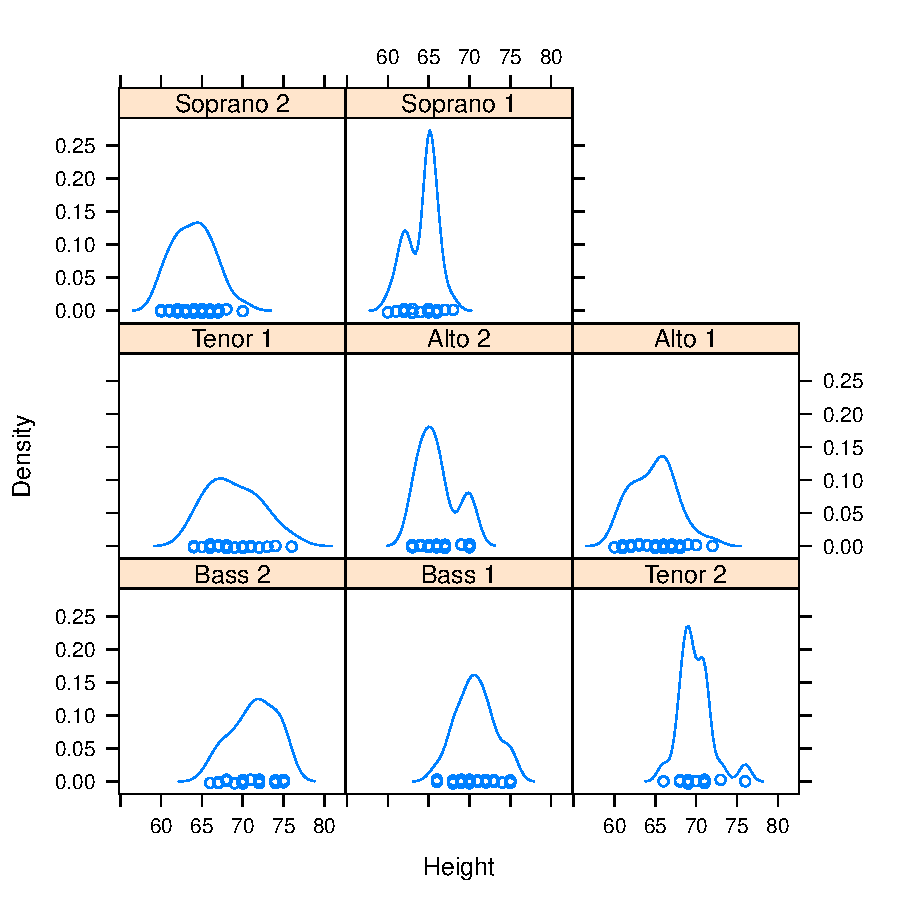
\includegraphics{rtf-025}

\begin{Schunk}
\begin{Sinput}
> addTrellisObject(rtf,trellis.object=p2,width=5,height=5,res=300)
\end{Sinput}
\end{Schunk}


\begin{Schunk}
\begin{Sinput}
> p3<-xyplot(uptake ~ conc | Plant, CO2, layout = c(2,2))
> print(p3) # note this is a multipage lattice plot
>           # but Sweave only shows the first plot
\end{Sinput}
\end{Schunk}
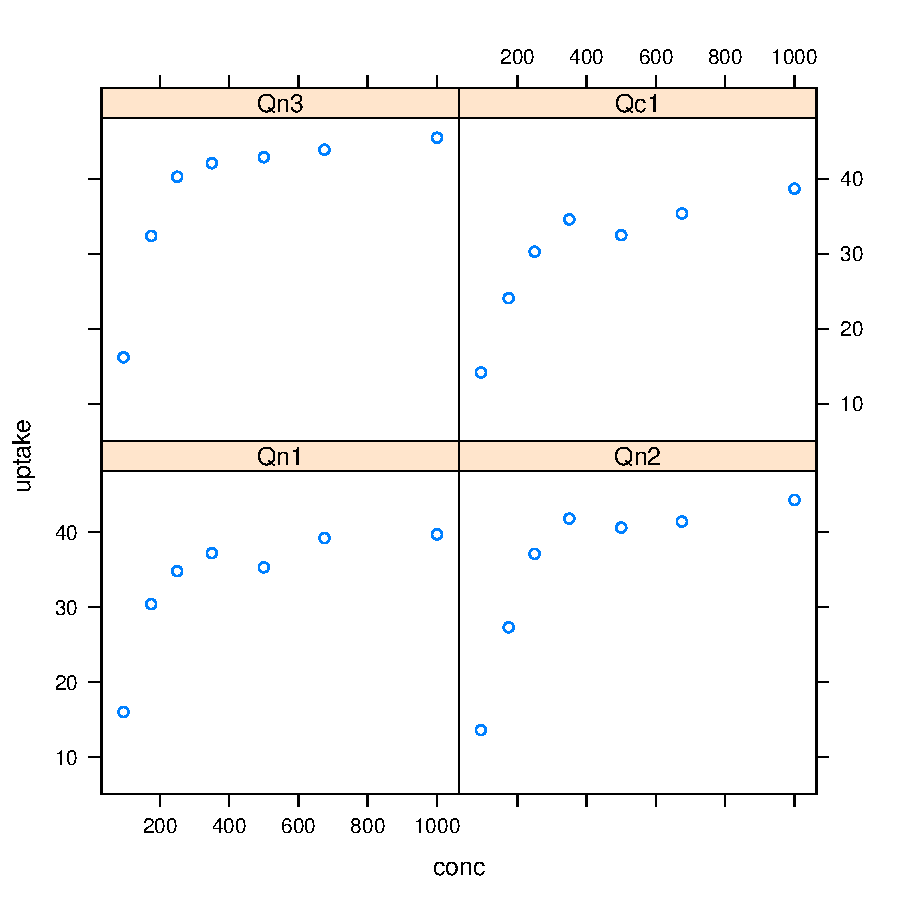
\includegraphics{rtf-027}

\begin{Schunk}
\begin{Sinput}
> addTrellisObject(rtf,trellis.object=p3,width=6,height=6,res=300)
\end{Sinput}
\end{Schunk}


\subsection{\texttt{ggplot2} Plots}
The \texttt{ggplot2} package is an alternative to \texttt{base} and \texttt{lattice} graphics and is an implementation of Leland Wilkinson's Grammar of Graphics.  Below is code that creates a simple \texttt{ggplot2} plot and stores a representation in a variable called, \texttt{mt}.  The \texttt{print} function may then be used to visualize the plot.

\begin{center}
\begin{Schunk}
\begin{Sinput}
> # plot
> library(ggplot2)
> mt <- ggplot(mtcars, aes(mpg, wt, colour = factor(cyl))) + geom_point()
> print(mt)
\end{Sinput}
\end{Schunk}
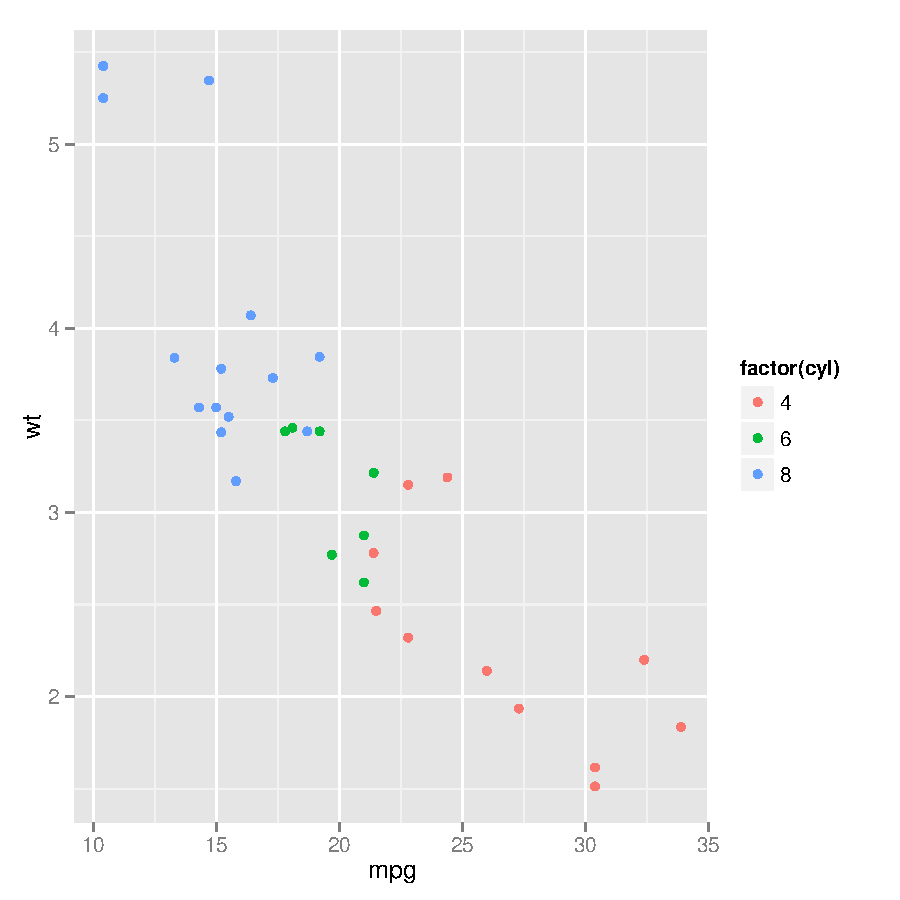
\includegraphics{rtf-029}
\end{center}


To include this plot in the RTF document we again call the \texttt{addPlot} method.  Just as with \texttt{lattice} trellis plots, we pass \texttt{print} as the \texttt{plot.fun} function and use the \texttt{mt} variable as a parameter for this function.


\begin{Schunk}
\begin{Sinput}
> addPlot(rtf,plot.fun=print,width=5,height=4,res=300, mt)
\end{Sinput}
\end{Schunk}


\subsection{External Figures}
The \texttt{rtf} package also supports incorporation of existing PNG images generated by \texttt{R} or any other software.  The code below demonstrates how to do this by pointing to the image file and specifying the desired output size.

\begin{Schunk}
\begin{Sinput}
> addPng(rtf, "foo.png", width=5, height=5)
\end{Sinput}
\end{Schunk}


\section{Table of Contents}
The \texttt{rtf} package also supports creation of a Table of Contents.  This uses the TOC.level attribute of headers throughout the RTF document.  Note that some word processors, including Microsoft Word, will not automatically render the table of contents unless the field is updated.  When opening the file for the first time in Microsoft Word, it may be necessary to force the field to update by right clicking on it and choosing 'Update Field'.

\begin{Schunk}
\begin{Sinput}
> addHeader(rtf,"Table of Contents")
> addTOC(rtf)
> addHeader(rtf,"Section 3",TOC.level=1)
> addHeader(rtf,"Section 3A",TOC.level=2)
> addHeader(rtf,"Section 3B",TOC.level=2)
\end{Sinput}
\end{Schunk}


\section{Output}
When an RTF document is complete, you close and write the document with the \texttt{done} command.  It may take some time to run depending on the document complexity and number of figures.  It is also customary to include information about the \texttt{R} session in reports.  For this we use the \texttt{addSessionInfo} method.  For example, the following code creates a page break, adds nicely formatted session information, and writes the RTF document.

\begin{Schunk}
\begin{Sinput}
> addPageBreak(rtf, width=8.5, height=11, omi=c(1,1,1,1))
> addSessionInfo(rtf)
> done(rtf)
\end{Sinput}
\end{Schunk}



\end{document}
